\section{Proof}

Now we are ready to prove the main result.

\begin{theorem}[{\cite[Theorem A]{calegari2024linear}}]
\label{thm:irrational}
$$
    L(2, \chi_{-3}) = \frac{1}{1^2} - \frac{1}{2^2} + \frac{1}{4^2} - \frac{1}{5^2} + \frac{1}{7^2} - \frac{1}{8^2} + \cdots
$$
is irrational. 
Moreover, $1, \zeta(2), L(2, \chi_{-3})$ are $\bQ$-linearly independent.
\end{theorem}

\begin{proof}
Assume $\bQ$-linear independence of $1, \zeta(2), L(2, \chi_{-3})$, so that there exist $a, b, c \in \bQ$ not all zero satisfying \eqref{eqn:lindep}.
As we mentioned before, this give 14 power series in $y$ that are $\bQ(y)$-linearly independent.
The denominator types of these series can be found in the below Table \ref{tab:denom} (we saw how the denominator types change under the symmetrization maps $\Sym^{\pm}$ from Daniel's talk - see \cite[Lemma 9.0.3]{calegari2024linear}).
The corresponding arrays $\mathbf{b}$ and $\mathbf{e}$ are
\begin{align*}
    \mathbf{b} &:= \begin{pmatrix}
        0 & 2 & 2 & 2 & 2 & 2 & 2 & 2 & 2 & 2 & 2 & 2 & 2 & 2 \\
        0 & 0 & 0 & 2 & 2 & 2 & 2 & 2 & 2 & 2 & 2 & 2 & 2 & 2
    \end{pmatrix}^\intercal \\
    \mathbf{e} &:= (0, 0, 1, 0, 0, 0, 0, 0, 0, 1, 1, 1, 1, 1).
\end{align*}
% \newpage

% \footnotesize
\begin{table}[t]
    \centering
    \begin{tabular}{ c|c } 
    function & denominator type \\
    \midrule
    \midrule
    $B_1$ & $1$ \\
     \midrule
    $B_2$ & $[1, \dots, 2n]$ \\
     \midrule
    $B_3$ & $n [1, \dots, 2n]$ \\
     \midrule
    $B_4$ & $[1, \dots, 2n]^2$\\
     \midrule
    $B_5$ & $(2n-1)[1, \dots, 2n]$\\
     \midrule
    $G$ & $[1, \dots, 2n]^2$ \\
     \midrule
    $G'$ & $[1, \dots, 2n+2]^2$ \\
     \midrule
    $G''$ & $[1, \dots, 2n+4]^2$ \\
     \midrule
    $G'''$ & $[1, \dots, 2n+6]^2$ \\
     \midrule
    $B_6$ & $n[1, \dots, 2n]^2$ \\
     \midrule
    $B_7$ & $n[1, \dots, 2n]^2$ \\
     \midrule
    $\int G(y) \dd y$ & $n[1, \dots, 2n-2]^2$ \\
     \midrule
    $\int \frac{G(y) - G(0)}{y} \dd y$ & $n[1, \dots, 2n]^2$ \\
     \midrule
    $\int \frac{G(y) - G(0) - G'(0)y}{y^2} \dd y$ & $n[1, \dots, 2n+2]^2$ \\
    \end{tabular}
    \caption{Denominator types}
    \label{tab:denom}
\end{table}


One can check analyticity (meromorphicity) of the pullbacks $\varphi^\ast F$ when $F$ is one of the series above, by applying Proposition \ref{prop:pullbackhol} with $\Sigma_{Y_0(2)}^0 = \{-\frac{1}{72}\}, \Sigma_{Y_0(2)}^1 = \emptyset, \varphi_{Y_0(2)} = \varphi$, and $U_{Y_0(2)}$ a sufficiently small open neighborhood of the line segment $[-\frac{1}{72}, 0]$, so we can apply Theorem \ref{thm:bound}.
(We also know that these have finite local monodromy of order dividing 2 at $y = 4$ by \cite[Lemma 9.0.3]{calegari2024linear}.)
We can compute $\tau(\mathbf{b}; \mathbf{e})$ explicitly, which is
$$
    \tau(\mathbf{b}; \mathbf{e}) = \tau^\flat(\mathbf{b}) + \tau^\sharp(\mathbf{e}) = \frac{191}{49} + \frac{27}{80} = \frac{16603}{3920} = 4.235459\dots.
$$
(For $\tau^\sharp(\mathbf{e})$, Figure \ref{fig:Igraph} shows the plot of the corresponding function $\xi \mapsto \frac{6\xi + I_{\xi}^{14}(\xi)}{98}$ which attains the minimum value of $\frac{27}{80}$ when $\xi \in [2, \frac{13}{6}]$).

\begin{figure}
    \centering
    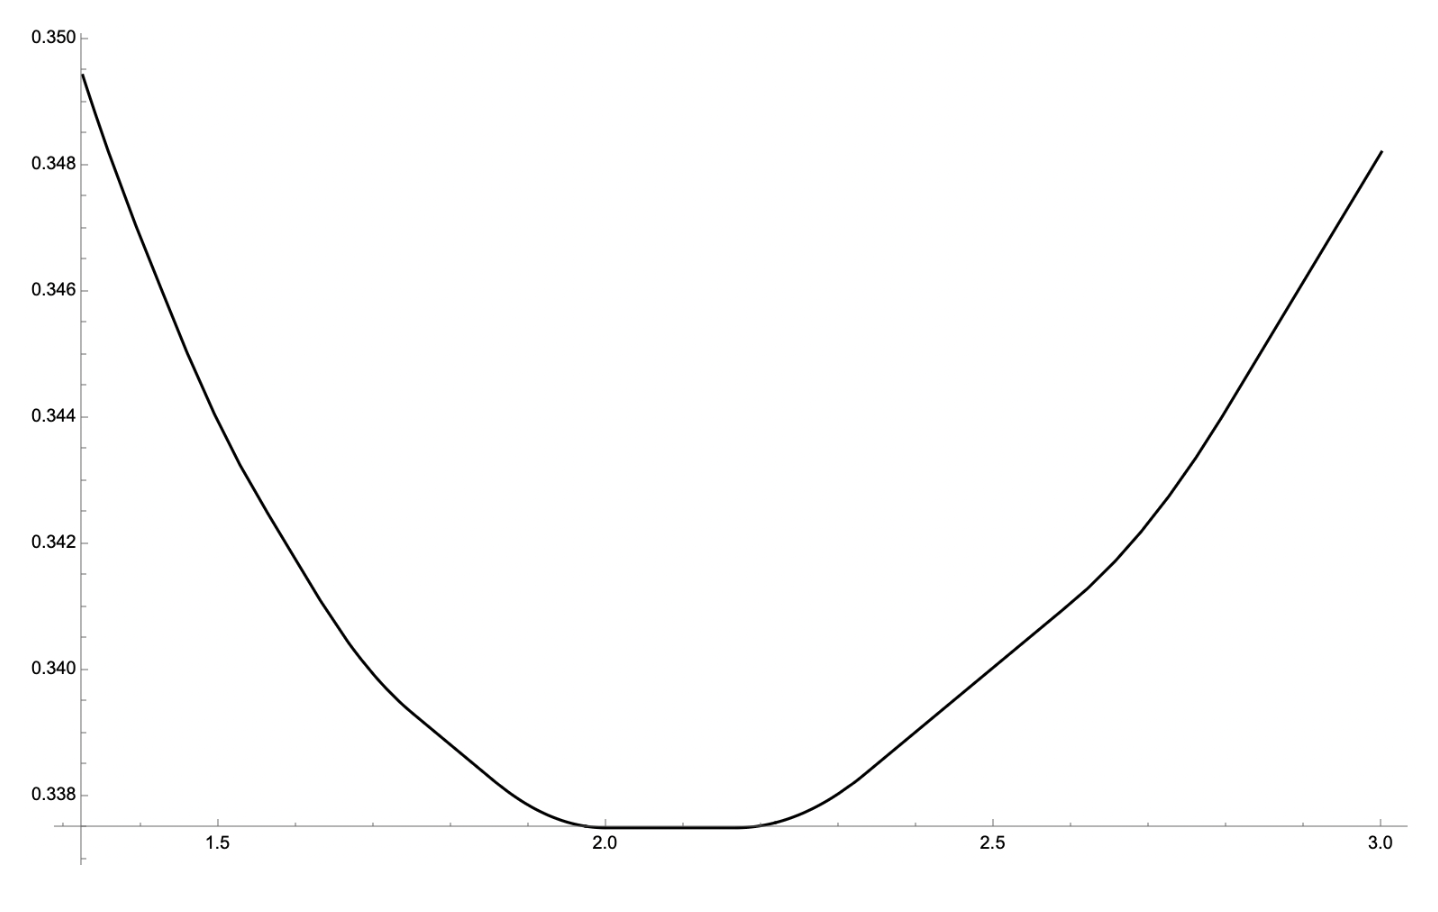
\includegraphics[width=0.8\linewidth]{src/Igraph.png}
    \caption{Plot of $\xi \mapsto \frac{6 \xi + I_{\xi}^{14}(\xi)}{98}$ on $[1.325, 3]$ \cite[Figure 13.0.3]{calegari2024linear}}
    \label{fig:Igraph}
\end{figure}

By definition of $\psi$ from Section \ref{sec:psi} (Equation \eqref{eqn:psi}), we have
$$
    |\varphi'(0)| = 256 \cdot c' \cdot R \cdot \frac{c^2 - 1}{c^2 + 1} \prod_{i=1}^{4} \frac{4r_i}{(1 + r_i)^{2}} = \frac{5448339453535586608000000000}{8658833407565631122430056127}.
$$
For the numerator, we can (numerically) compute the double integral with the explicit formula of $\varphi(z) = h(\psi(z))$, which gives
$$
    \iint_{\bT^2} \log |\varphi(z) - \varphi(w)| \dd \mu(z) \dd \mu(w) = 11.844\dots.
$$
Hence we get a holonomy bound
$$
    m \le \frac{11.845}{\log \left(\frac{5448339453535586608000000000}{8658833407565631122430056127}\right) - \frac{11603}{3920}} =13.9938 \dots < 14
$$
and get a contradiction.
\end{proof}

\begin{remark*}
You may found that the denominator types in Table \ref{tab:denom} are slightly larger than the numbers recorded in $\mathbf{b}$.
For example, $G'(y)$ has a denominator type of $[1, \dots, 2n + 2]^2$, not $[1, \dots, 2n]^2$.
This is not a problem, since one can replace it by $[1, \dots, (2 + \epsilon)n]^2$ for sufficiently small $\epsilon > 0$ for all but finitely many $n$'s, and the finite initial terms can be made to have any given denominator type by scaling, which yields the same bound as $\epsilon \to 0$ \cite[Remark 6.0.12]{calegari2024linear}.
\end{remark*}

\begin{remark*}
If we want to stick with a version of the theorem with $\mathbf{e} = \mathbf{0}$, one needs to append $\mathbf{e}$ to $\mathbf{b}$ (which is equivalent to replace $n^e$ with $[1, \dots, n]^e$ and get
\begin{align*}
    \mathbf{b}' := \begin{pmatrix}
        0 & 2 & 2 & 2 & 2 & 2 & 2 & 2 & 2 & 2 & 2 & 2 & 2 & 2 \\
        0 & 0 & 0 & 2 & 2 & 2 & 2 & 2 & 2 & 2 & 2 & 2 & 2 & 2 \\
        0 & 0 & 1 & 0 & 0 & 0 & 0 & 0 & 0 & 1 & 1 & 1 & 1 & 1
    \end{pmatrix}^\intercal 
\end{align*}
However, we cannot directly apply Theorem \ref{thm:bound} since the appended column is not in an increasing order.
In this case, one has a more general result \cite[Theorem 8.0.1]{calegari2024linear} allowing such relaxations at the cost of a worse bound.
We need to replace $\tau^\flat(\mathbf{b}) + \tau^\sharp(\mathbf{e})$ with $\tau^{\flat\flat}(\mathbf{b}')$ (where the definition can be found in \cite[Equation 8.0.2]{calegari2024linear}), which is at least
$$
    \tau^{\flat\flat}(\mathbf{b}') \ge \frac{884}{196} = 4.510\dots,
$$
significantly worse than the above $\tau(\mathbf{b};\mathbf{e}) = 4.2354\dots$ and not enough to get a dimension bound less than 14.
\end{remark*}

\begin{remark*}
One may not happy about the possible numerical issue when we compute the double integral.
The authors used \texttt{mathematica} to estimate the integral, and the formula of $h(q)$ and $\psi(x)$ are explicit enough to estimate the integral as accurately as we want.
Alternatively, there are two other holonomy bounds (Theorem 6.0.2 and Theorem 7.1.6 of \cite{calegari2024linear}) which are much more complicated but gives a better numerical stability, and strong enough to yield similar contradictions.
\end{remark*}